% !TEX TS-program = pdflatex
% !TEX root = ../ArsClassica.tex
\newcommand{\bpic}{$\beta$ Pic b }
\newcommand{\mj}{M$_{j}$}
%************************************************
\chapter{Introduction}
%Meyor queloz
Since the first detection of a planet around a sun-like star \parencite{Mayor1995} the field of exoplanets has evolved rapidly.
Thousands of companions have been identified using the radial velocity and transit detection methods, and a handful have been imaged directly using both ground and space based observatories.
In the last decade, many advances have been made that allow us to begin to characterize the properties of a few of these planets using spectroscopy.
With the launch of the James Webb Space Telescope (JWST) in 2021, and the dawn of the era of extremely large telescopes, we will be able to peer deeper into these planets and further constrain atmospheric or geological properties, allowing us to answer questions about their formation history, climate, and even the prospects for habitability and life.

JWST will operate in near to mid infrared wavelengths, which will provide a new window into studying the atmospheres of exoplanets and brown dwarfs. 
The Mid Infrared Instrument (MIRI) will provide unprecedented spectral resolution in the mid infrared, allowing for the measurement of composition, pressure and temperature. 
Novel instrumentation does not come without challenges. 
Optical and instrumental effects will constrain the ability to which we can measure spectral features, which will ultimately limit the science that can be accomplished.

In this thesis, we will measure the impact of thin-film fringing in the layers of the detectors in the MIRI Medium-Resolution Spectrometer on measurements of atmospheric parameters of brown dwarfs and exoplanets.
This will provide a baseline for determining the level of correction necessary to minimize the impact of fringing, as well as providing a first look into the ability of the MRS to characterize atmospheres.

\section{Exoplanets}
The last quarter century of observations has revealed the diversity of exoplanets and extra-solar systems.
Both the architecture and individual planetary characteristics vary greatly when compared to each other, as well as to our own solar system.
From the hot Jupiters initially found by Mayor and Queloz \parencite{Mayor1995} to the thousands of planets discovered by the Kepler mission, the variety in exoplanets has raised questions about their formation and development, as well as their present day structure, climate, and even prospects for life.
Improvements to observational techniques have allowed us to improve our understanding of these planets.
Secondary eclipse and transmission spectroscopy has opened the door to the study of planets in close orbits to their host stars, while emission spectroscopy of young planet has allowed for constraints on models of planet formation.
Over the next decades, new instruments will be developed that improve sensitivity, allowing us to study smaller, colder and fainter planets: with the ultimate goal of studying atmospheric and surface features of an earth-like planet.

Of particular interest are observable features that allow us to measure physical properties of exoplanets.
The radial velocity (RV) method provides a measure of the planet mass, while a transit can constrain the radius.
Already these properties tell us something about the overall structure of the planet.
Spectroscopy can provide insight into the composition of the planet's atmosphere, as well as its temperature and pressure.
These properties are linked to its age and location of formation in the circumstellar disk.
The atmosphere, combined with the distance between the planet and its star determine the climate of the planet.

%Exoplanet Science Strategy Text: state of field, goals, timelines, summary of methods, biosignatures, formation, tracers, methods, parameters of interest.
% Kepler, Tess, Cheops, RV
\subsubsection{Direct Imaging}
While the majority of exoplanet detections have been made using the radial velocity or transit techniques, direct imaging opens up the possibility of collecting light from the planet itself.
This provides a window into the planet's atmosphere and surface.
Most direct imaging to date has used near-to-mid infrared wavelengths, where the contrast between the thermal emission from the planet and the star is at a minimum.
This has its drawbacks: we are so far only able to image young planets that have retained some of the heat from their formation.
 
\begin{figure}[t]
	\centering
	\includegraphics[width=0.75\linewidth]{familyphoto.png}
	\caption{A family portrait of some of the directly imaged exoplanets.
	\parencite{Marois2010,Rameau2013,Stolker2020,Sallum2015,Keppler2018,Currie2018,Macintosh2015,Chauvin2004,Quanz2010}.}
\end{figure}

Direct imaging can make use of both ground and space based observatories. 
However, the high spatial resolution required drives the need for a large primary mirror, limiting the possibilities of space-based telescopes. On the other hand, atmospheric turbulence necessitates the use of an adaptive optics equipped facility to observe from the ground. 
Atmospheric absorption due to telluric lines (absorption lines of Earth's atmosphere) also restrict infrared observations to narrow bands.

In addition to the requiring high spatial resolution, it is also challenging to separate the light emitted by the planet from that of the star.
Imaging techniques such as Angular Differential Imaging (ADI) \parencite{Marois2007} and Reference Differential Imaging (RDI) \parencite{Lefreniere2009,Soummer2012} provide methods for reducing the stellar point-spread-function (PSF). %\parencite{Macintosh2006} %ADI
Coronagraphs are optical elements which suppress the stellar PSF through self-destructive interference or physical occultation, depending on the position in the optical path.
The difference in spectra between the planet and the star can also be used to separate the two sources.


Presently, 10m class telescopes such as the Very Large Telescope (VLT) in Paranal, Chile or the Gemini Observatory split between Hawaii and Chile provide the best combination of resolution and instrumentation to perform direct imaging of exoplanets.
The NACO instrument at the VLT provided the first image of an exoplanet in 2004 \parencite{Chauvin2004}.
These observatories are among those equipped with an adaptive optics system, corongraphic instrumentation and near to mid infrared imaging and spectroscopic capabilities to directly image exoplanets, with several exemplar systems becoming standard objects of interest.
While it's terribly interesting to explore the details of each of these objects, we will focus our discussion on objects will be used further in this study, due to their scheduled observation as part of the JWST GTO and Early Release Science (ERS) programs \parencite{Beichman2019}. 
The parameters of these and other directly imaged exoplanets and brown dwarfs are summarized in table \ref{tab:exoplanetparams}. 
 %Not 2019 - summary of JWST science and instruments
\parencite{Lagage2015} %Exoplanet characterization with JWST MIRI white paper
\subsubsection{VHS 1256 b}
\begin{wrapfigure}{r}{5.8cm}
	\vspace{-1em}
	\centering
	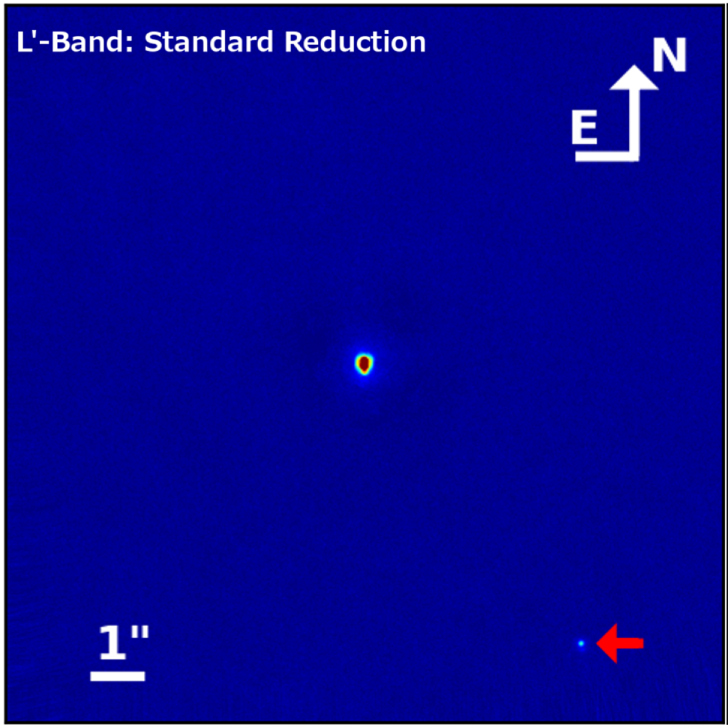
\includegraphics[width=5cm]{vhs1256b.jpg}
	\caption{VHS-1256b as observed with Subaru/IRCS in the L'-band \parencite{Rich2016}, reduced using the LOCI algorithm \parencite{Galicher2011}.}
	\vspace{-1em}
\end{wrapfigure}
Originally discovered in 2015 \parencite{Gauza2015} as part of the VISTA Hemisphere Survey, VHS-1256b is a late-L dwarf in a 102 AU orbit around an M dwarf.
\parencite{Gauza2015} present astrometric, photometric and spectroscopic data on the planet, finding an age of 150-300 Myr from a moving group association, a luminosity log($L_{bol}/L_{\odot}$) of -5.05$\pm0.22$ and infer a mass of 11.2$^{+9.2}_{-1.8}$ M$_{Jup}$. 
The effective temperature is found to be 880$^{+140}_{-110}$ K from evolutionary models. 
This is substantially colder than field dwarfs of a similar spectral type (typically 1400K), and so it is proposed that a thick Fe and Mg-Si cloud layer acts to reduce the effective temperature.
Similar findings are presented by \parencite{Rich2016} using Subaru/IRCS.

In \parencite{Miles2018}, methane is detected using KECK/NIRSPEC in the L-band. 
The shallow depth of the feature indicates chemical disequilibrium in the photosphere, as the derived abundance departs from an equilibrium abundance by a factor of 10-100.
However, the best fit model retrieves substantially different parameters for temperature (1240 K) when compared to previously published results.

The wide separation (8") and proximity to Earth make VHS-1256b an ideal target for studying atmospheric properties.
It will be observed as part of the JWST ERS Program \parencite{Hinkley2019}, where a medium resolution spectrum (R$\geq$1700) will be measured from 0.6-28 micron. 
This will enable a more precise measurement of the abundance of methane and other species in the atmosphere, and will allow for investigation of the cloud properties in the mid infrared.
\subsubsection{2M1207b}
\begin{landscape}
	\begin{table}[t]
		\centering
		\begin{small}
			\begin{tabular}{lllllllll}
				\toprule
				%Name, Mass, Luminosity, Age, Separation, Sep AU, Pri Mass
				\textbf{Name} & \textbf{d [pc]} & \textbf{Mass [M$_{jup}$]} & \textbf{Sep [au]} & \textbf{Sep ["]} & \textbf{Age [Myr]} & \textbf{log(L$_{bol}$/L$_{\odot}$)} & \textbf{T$_{eff}$ [K]} & \textbf{References}\\
				\midrule
				\multicolumn{9}{c}{\textbf{Widely separated companions}}\\
				\midrule
				VHS 1256b & $12.7\pm1.0$  & $2\pm1$     & $102$ & $8.1$ & $10^{3}-10^{4}$ & $-5.05\pm0.22$ & $880$ & \parencite{Gauza2015}\\
				Fomalhaut b & $7.704\pm0.028$ & $\leq 2$ & $119$ & $13$ & $440\pm40$ & \ldots & $1600\pm100$ &\\
				\midrule
				\multicolumn{9}{c}{\textbf{Close in companions}}\\
				\midrule
				2M1207b   & $152.4\pm1.1$ & $2\pm1$     & $41$ & $0.8$ & $10\pm3$ & $-4.68\pm0.05$ & $1600\pm100$ &\\
				51 Eridani b & $29.4\pm0.3$ & $2\pm1$   & $13$ & $0.45$ & $23\pm3$ & $-5.06\pm0.2$ & $700$ &  \parencite{Macintosh2015}\\
				\bpic     & $19.3\pm0.2$  & $2\pm1$     & $9$ & $0.4$ & $23\pm3$ & $-3.78\pm0.03$ & $1600\pm100$ & \parencite{Quanz2010}\\
				GJ 504b   & $17.56\pm0.08$  & $3-30$    & $44$ & $2.5$ & $100-6500$ & $-6.13\pm0.03$ & $544$ & \parencite{Skemer2016}\\
				HD 95086b & $90.4\pm3.3$  & $5\pm2$     & $56$ & $0.6$ & $17\pm4$ & $-4.96\pm0.10$ & $1050$  &\parencite{DeRosa2016}\\	
				HR8799b   & $39.4\pm1.0$  & $5\pm1$     & $68$ & $1.7$ & $40\pm5$ & $-5.1\pm0.1$ & $870^{+30}_{-70}$ & \parencite{Marois2008,Skemer2012}\\
				HR8799c   & $39.4\pm1.0$  & $7\pm2$     & $38$ & $0.95$ & $40\pm5$ & $-4.7\pm0.1$ & $1090^{+10}_{-90}$ &\parencite{Marois2008,Skemer2012}\\
				HR8799d   & $39.4\pm1.0$  & $7\pm2$     & $24$ & $0.62$ & $40\pm5$ & $-4.7\pm0.2$ & $1090^{+10}_{-90}$ &\parencite{Marois2008,Skemer2012}\\
				HR8799e   & $39.4\pm1.0$  & $7\pm2$     & $14$ & $0.38$ & $40\pm5$ & $-4.7\pm0.2$ & $1000$ &\parencite{Marois2008,Skemer2012}\\	
				LkCa 15b  & $145\pm15$    & $6\pm4$     & $20$ & $0.08$ & $2\pm1$ & \ldots & \ldots &\\
				PDS 70b   & $113.43\pm0.52$ & $7\pm2$   & $23$ & $0.19$ & $5\pm1$ & \ldots & $900$ &\parencite{Haffert2019}\\
				PDS 70c   & $113.43\pm0.52$ & $4.4\pm1$ & $30$ & $0.24$ & $5\pm1$ & \ldots &  $10^{4}$ & \parencite{Haffert2019}\\
				\midrule
				\multicolumn{9}{c}{\textbf{Nearby Brown Dwarfs}}\\
				\midrule
				WISE 0855   & $2.2\pm0.2$ & $3-10$ & \ldots & \ldots & $10^{3}-10^{4}$ & $-10.5$ &  $225-260$ & \parencite{Luhman2014,Tinney2014}\\
				Luhman 16B   & $1.998\pm0.0004$ & $28.6\pm0.3$ & \ldots & \ldots & $600-800$ & $-4.68$&  $1201$ & \parencite{Sahlmann2015,Garcia2017}\\
				\bottomrule
			\end{tabular}
		\end{small}
		\caption{Summary of directly imaged planet and brown dwarf parameters based on \parencite{Bowler2016} and references therein. Luminosity for WISE 0855 is calculated in H band.}
		\label{tab:exoplanetparams}
	\end{table}
\end{landscape}
\section{Brown Dwarfs}
\parencite{Oliveira} %BDs with JWST
\parencite{Helling2014}% Brown dwarf atmospheres
\parencite{Cooper2014} %Brown dwarf clouds/cloud formation
\parencite{Madhusudhan2018a} %BD observations/atmospheres
\parencite{Burrows2003} % Brown dwarf models/spectra coolest dwarfs
\parencite{Marley2014} %Modelling brown dwarf and giant planet atmospheres
\parencite{Manjavacas2014} %Thesis - physical characterization of brown dwarfs
\parencite{Biller2017} %Variability in time for BDs
\parencite{Faherty2018} % Water clouds in cold BDs
\parencite{Morley2014} %Water clouds in Y dwarfs and exoplanets

\subsection{Physics}
\subsection{Observational Properties}
\subsubsection{T-Type}
\subsubsection{L-Type}
\subsubsection{Luhman 16B}
\subsubsection{Y-Type}
\subsubsection{WISE 0855-0714}

\section{Motivation}
\subsection{Current Status of Atmospheric Characterization}
Both exoplanets and brown dwarfs raise interesting questions, but the real challenge is in gathering and processing the data necessary to answer them. 
The best methods currently in use involve taking spectroscopic data and inferring atmospheric properties from the spectral features.
The light we measure may be thermal emission from the planet, where it is absorbed and scattered as it passes through the planet's atmosphere, or it may be light from the planet's host star which passes through the upper layers of the atmosphere.
These provide complementary information about the composition and structure of the atmosphere, probing different altitudes and pressures.
While a more complete overview of exoplanet atmospheres is covered in the literature \parencite{Bozza,Madhusudhan2014,Seager2010}, we will briefly summarize the current methods used and what has been learned so far.
%Transmission spectroscopy, facilities, atmosphere, climate, condensates
 % Exoplanet atmosphere measurements, hr8799 photometry/spec, prospects for jw
 %Exoplanet atmospheres textbook: observation, models, spectroscopy, solar system atmospheres
 %Atmospheric char with MIRI (coron,LRS, not MRS I think)
%\parencite{Madhusudhan2016} %Chemistry, Formation, Habitabiltiy
\subsubsection{Transmission Spectroscopy}
\parencite{Kreidberg2018}
\parencite{Lee2012} % HD189733b trans spec
\parencite{MacDonald2017} % Nitrogen chem, HD209458b
\parencite{Madhusudhan} %Wasp12b need year
\subsubsection{Emission Spectroscopy}
\parencite{Biller2018}
\parencite{Danielski2018}
\parencite{GRAVITYCollaboration2019}
\subsection{JWST Studies}
\parencite{Beichman2019} %JWST whitepaper on imaging/spec
\subsubsection{Early Release Science}
\subsubsection{GTO Programs}
\subsection{Biosignatures and Future Missions}
\section{Thesis Overview}
With sufficient background and motivation, we will now outline the remainder of this thesis.

Chapter 2 will provide a more extensive background of the James Webb Space Telescope, and in particular the MIRI Medium Resolution Spectrometer (MRS).
We will outline the principle optical components dedicated to integral field spectroscopy, as well as the detector characteristics of MIRI.
This will provide the necessary background to understand the instrumental and optical effects discussed in Chapter 3.

The third chapter examines the fringing effect in the MIRI MRS instrument.
We discuss the optical effects that result in fringing patterns, as well as outlining current and future strategies for fringe correction.
We describe the creation and processing of our mock observations using the MIRI instrumental simulator and the JWST data reduction pipeline.
With the degraded spectra from the simulated data, we measure the impact of fringing on spectral extraction using cross correlation techniques, and and how this impacts molecular mapping studies.
This in turn motivates Chapter 4, where the species identified using molecular mapping can justify the inclusion or exclusion of particular species in an atmospheric retrieval.

In Chapter 4 we explore atmospheric retrievals with the MIRI MRS.
We outline our procedure for performing a retrieval using the petitRADTRANS radiative transfer code and Multinest as an implementation of the nested sampling strategy for parameter space exploration
We measure the impact of fringing on parameter estimation, and also investigate how observing parameters will impact retrievals, discussing the advantages and challenges of studying atmospheres in the mid infrared.

Finally we summarize and discuss our finding and future investigations in the final chapter.

